\documentclass[tikz,border=4pt]{standalone}
\usetikzlibrary{positioning,arrows.meta,fit,backgrounds,calc}
\begin{document}
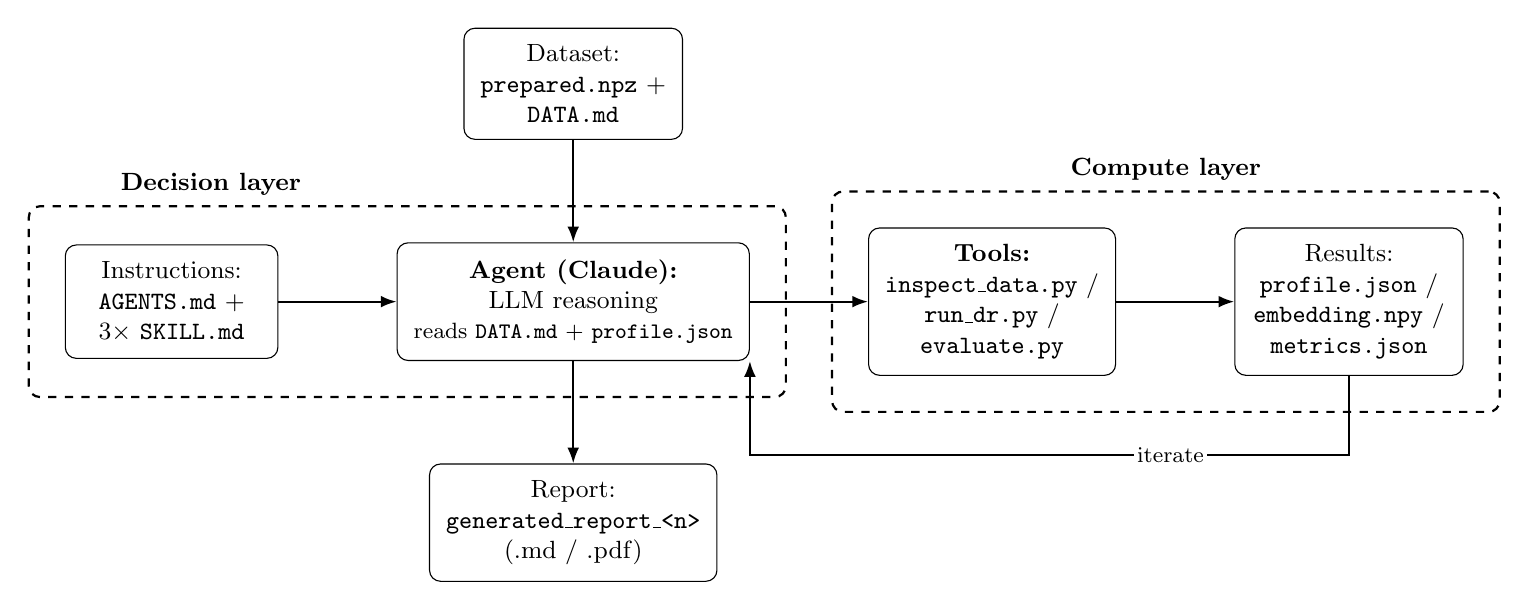
\begin{tikzpicture}[
  node distance=1.3cm and 1.5cm,
  box/.style={draw, rounded corners, align=center, minimum height=1.15cm, minimum width=2.7cm, font=\small, inner sep=6pt},
  arrow/.style={-{Latex[length=2mm]}, thick},
  layer/.style={draw, dashed, rounded corners, thick, inner sep=13pt}
]
\node[box] (agent) {\textbf{Agent (Claude):}\\ LLM reasoning\\ \footnotesize reads \texttt{DATA.md} + \texttt{profile.json}};
\node[box, above=of agent] (dataset) {Dataset:\\ \texttt{prepared.npz} +\\ \texttt{DATA.md}};
\node[box, left=of agent] (instructions) {Instructions:\\ \texttt{AGENTS.md} +\\ 3$\times$ \texttt{SKILL.md}};
\node[box, below=of agent] (report) {Report:\\ \texttt{generated\_report\_<n>}\\ (.md / .pdf)};
\node[box, right=of agent, minimum width=3.1cm] (tools) {\textbf{Tools:}\\ \texttt{inspect\_data.py} /\\ \texttt{run\_dr.py} /\\ \texttt{evaluate.py}};
\node[box, right=of tools, minimum width=2.9cm] (results) {Results:\\ \texttt{profile.json} /\\ \texttt{embedding.npy} /\\ \texttt{metrics.json}};

\begin{pgfonlayer}{background}
\node[layer, fit=(instructions)(agent), label={[font=\small]above left:\textbf{Decision layer}}] {};
\node[layer, fit=(tools)(results), label={[font=\small]above:\textbf{Compute layer}}] {};
\end{pgfonlayer}

\draw[arrow] (dataset) -- (agent);
\draw[arrow] (instructions) -- (agent);
\draw[arrow] (agent) -- (tools);
\draw[arrow] (tools) -- (results);
\draw[arrow] (agent) -- (report);
\draw[arrow] (results.south) -- ++(0,-1.0) -| (agent.south east);
\node[font=\footnotesize, fill=white, inner sep=1pt] at ($(tools.south)!0.5!(results.south) + (0,-1.0)$) {iterate};
\end{tikzpicture}
\end{document}
